\chapter[Resultados Alcançados]{Resultados Alcançados}\label{cap4}

\section{O Editor OGG}

O Editor de \textit{audiobooks} gera com sucesso um formato Ogg Vorbis com todos os metadados inseridos no pacote Vorbis de comentários e as marcações de conteúdo contidas no pacote LGMK construído. Mesmo com sua estrutura alterada, o formato *.ogg pode ser executado em players com suporte a estes arquivos como, a exemplo, o \textit{sox} ou Rhythmbox.

A efeito de comparação ao \cite{herbert}, cujo trabalho desenvolveu um formato parecido que não faz uso da compressão de dados, também foi utilizado o Hino Nacional Brasileiro para simular um \textit{audiobook}. O arquivo original no formato WAV possui 3 minutos e 41 segundos de duração e ocupa 42,5 MB de espaço em memória. Este arquivo foi carregado pelo Editor e em seguida foram inseridos metadados conforme mostra Tabela \ref{tab1}.

\begin{table}[ht]
\centering
\caption{Metadados inseridos no \textit{comment header}.}
\vspace{0.5cm}
\begin{tabular}{ll}

\hline
\textbf{Nome} & \textbf{Valor} \\
\hline
Título & Hino Nacional Brasileiro \\
Autor & Joaquim Osório \& Francisco Manuel \\
Idioma & Português \\
Editora & \\
Local de Criação & Brasil \\
Número de Páginas & 0 \\
Ano de Criação & 1822 \\
\hline

\end{tabular}
\label{tab1}
\end{table}

Para verificação dos metadados inseridos no pacote de comentários do formato Ogg, a Figura \ref{meta} apresenta a decodificação do arquivo utilizando a ferramenta ogg-dump. O pacote de comentários está identificado como pacote de número 1 e nele é possível notar que os metadados foram inseridos corretamente.

 \begin{figure}[ht]
	\centering
		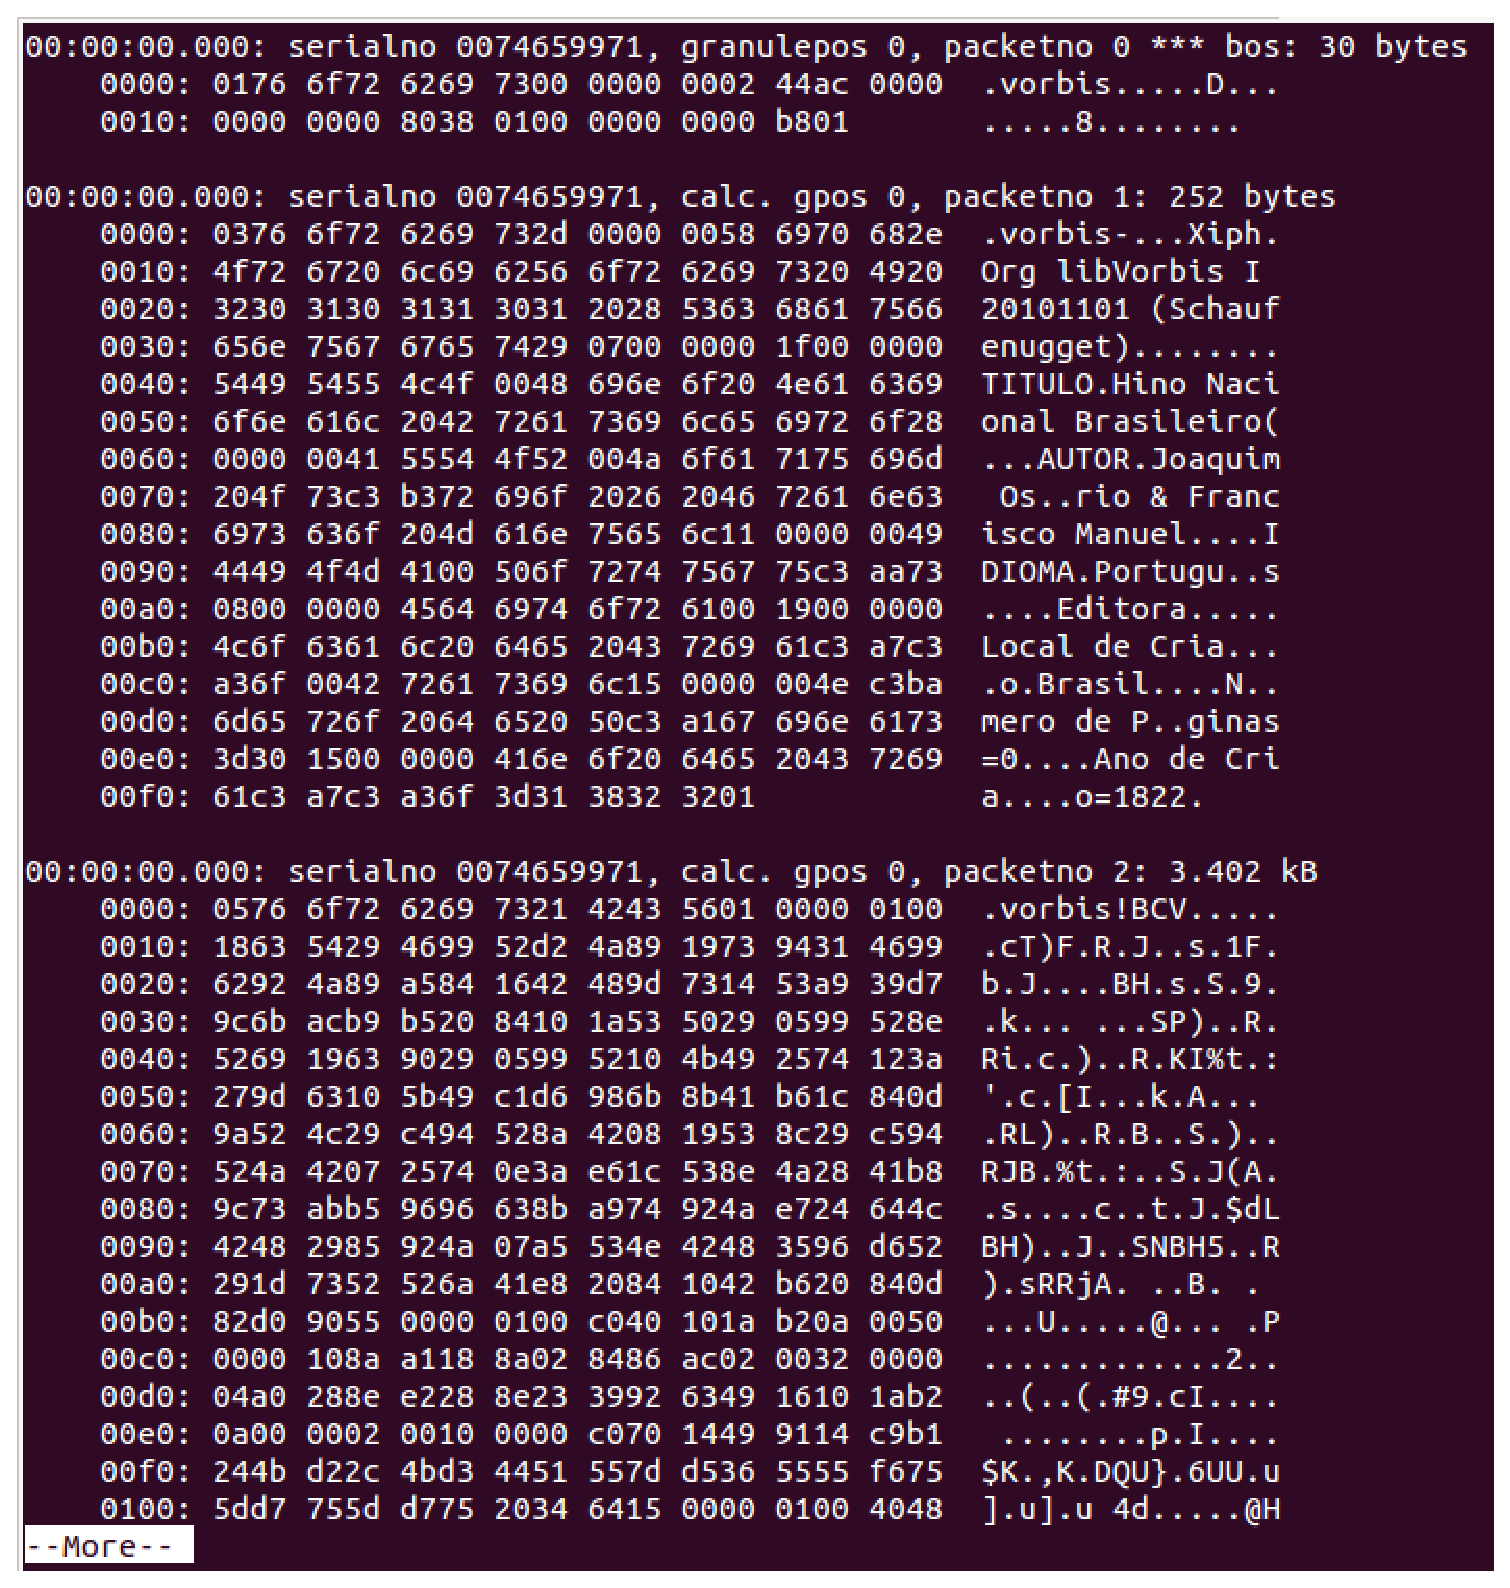
\includegraphics[keepaspectratio=true,scale=0.4]{figuras/hnbogg.eps}
	\caption{Utilização do oggz-dump - pacote de comentários.}
	\label{meta}
\end{figure}

Sobre as marcações de conteúdo, a Tabela \ref{mark} lista as informações inseridas no pacote LGMK. Cada item da tabela representa uma marcação composta por uma legenda e o tempo em que se deve estar posicionada.

\begin{table}[ht]
\centering
\caption{Marcações inseridas no \textit{LGMK header}.}
\vspace{0.5cm}
%\rowcolor{1}{}{lightgray}
\begin{tabular}{ll}

\hline
\textbf{Nome da Marcação} & \textbf{Tempo(s)} \\
\hline
Parte 1 & 0 \\
Parte 2 & 103 \\
Introdução 1 & 0 \\
Primeira Estrofe & 28 \\
Segunda Estrofe & 44 \\
Terceira Estrofe & 60 \\
Quarta Estrofe & 64 \\
Quinta Estrofe & 79 \\
Sexta Estrofe & 91 \\
Introdução 2 & 103 \\
Sétima Estrofe & 132 \\
Oitava Estrofe & 148 \\
Nona Estrofe & 164 \\
Décima Estrofe & 168 \\
Décima Primeira Estrofe & 183 \\
Décima Segunda Estrofe & 195 \\
Décima Terceira Estrofe & 201 \\
Final & 206 \\
\hline

\end{tabular}
\label{mark}
\end{table}

A verificação da inserção dos marcadores de conteúdo no pacote LGMK pode ser visualizado usando a ferramenta oggz-dump. A Figura \ref{lgmk} mostra o pacote LGMK que pode ser identificado pelo número de pacote 3 e sua descrição evidencia os marcadores de conteúdo que o compõe.

 \begin{figure}[ht]
	\centering
		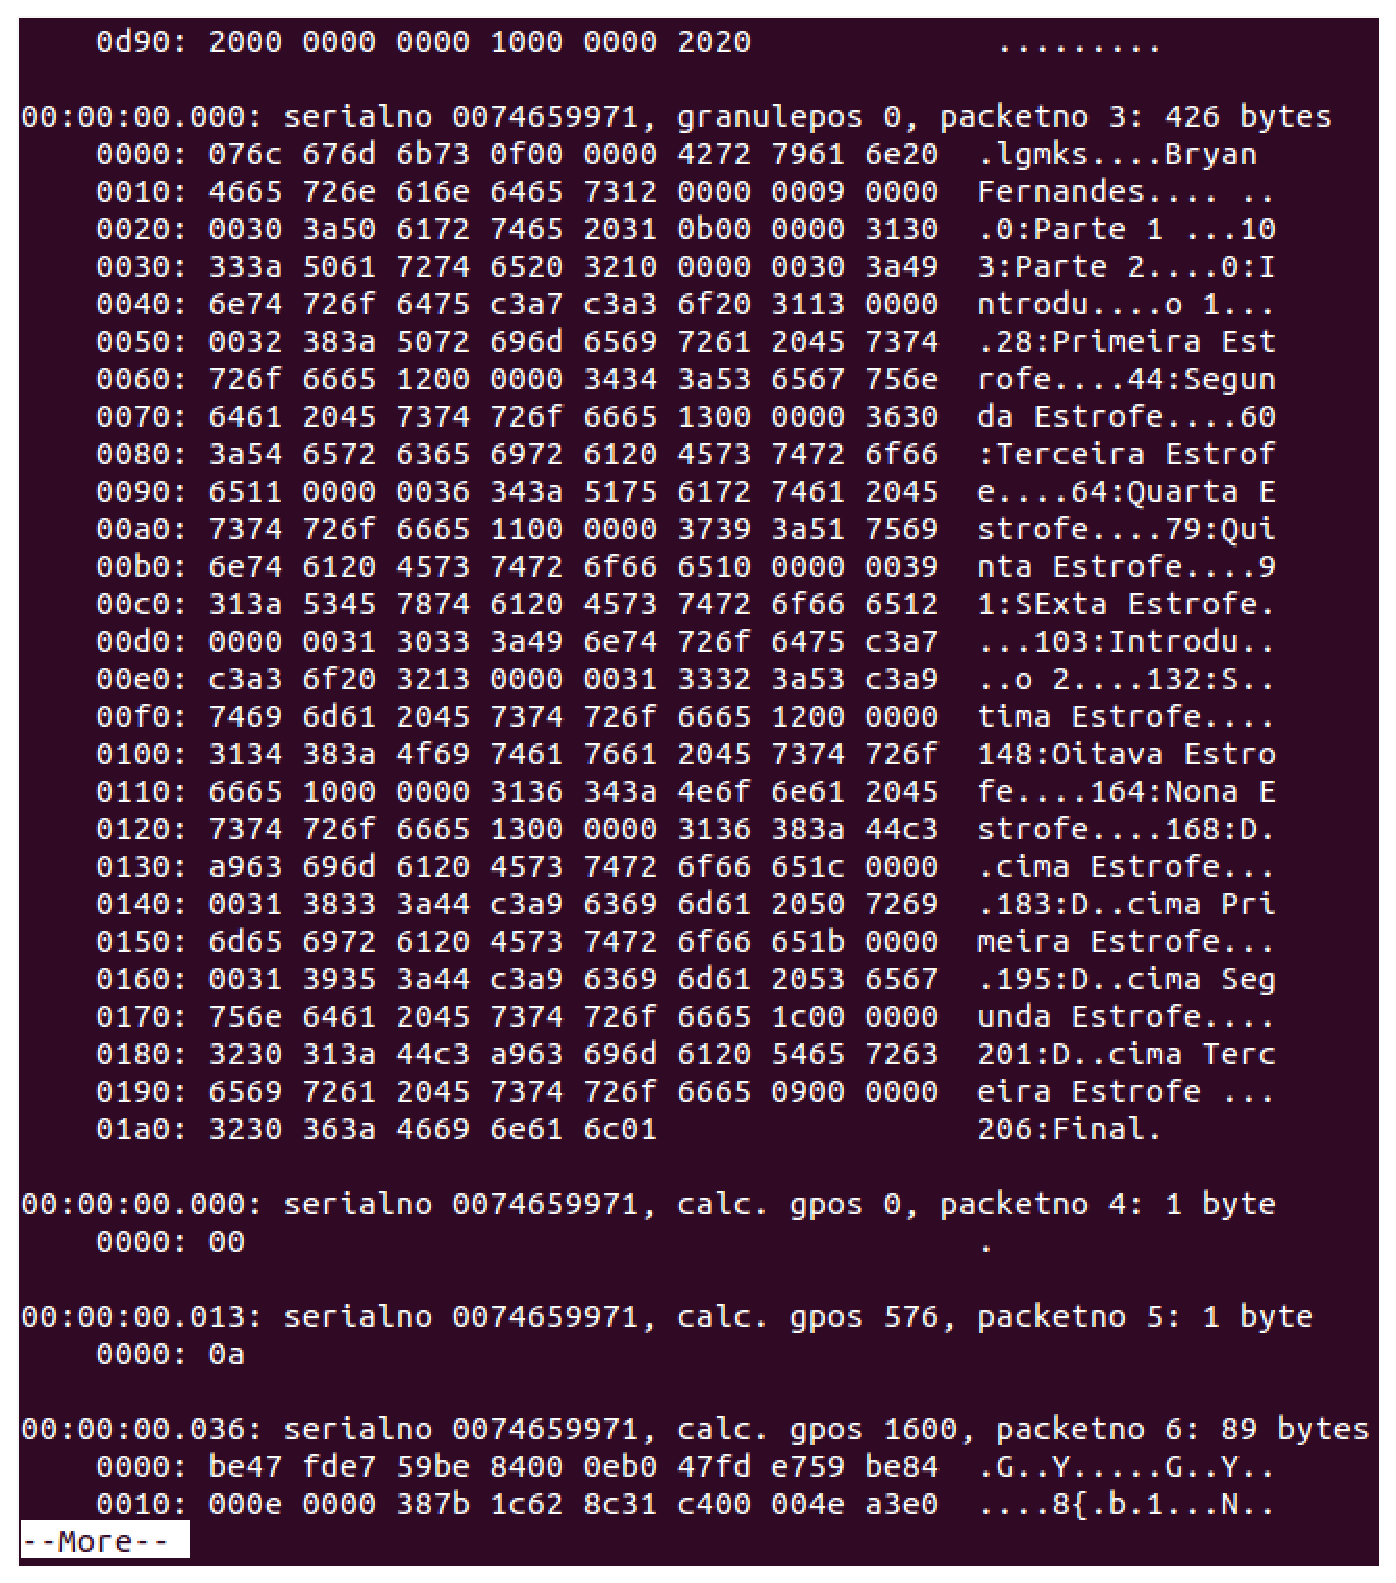
\includegraphics[keepaspectratio=true,scale=0.4]{figuras/hnblgmkogg.eps}
	\caption{Utilização do oggz-dump - pacote LGMK.}
	\label{lgmk}
\end{figure}

O pacote Ogg Vorbis gerado possui apenas 1,84MB e não mais 42,5MB como o arquivo original. Houve uma redução considerável devido ao algoritmo de compressão do \textit{codec} Vorbis. O arquivo gerado é executado corretamente do início ao fim sem interrupções. Também foi feito um teste para verificar se o pacote LGMK não iria corromper o arquivo Ogg Voribs ao inserir um número considerável de marcacões, um total de 22 milhões de marcações. O arquivo final ficou com 340MB de tamanho, no entanto, o player conseguiu executá-lo normalmente.


% O Editor também é capaz de decodificar todos os dados conforme mostra a Figura \ref{decodeogg}

% \begin{figure}[ht]
% 	\centering
% 		\includegraphics[keepaspectratio=true,scale=0.5]{figuras/decodeogg.eps}
% 	\caption{Utilização do Editor para decodificar os dados.}
% 	\label{decodeogg}
% \end{figure}

%1,86MB

\section{O Tocador}

O Tocador desenvolvido é capaz de executar o novo formato gerado pelo Editor OGG e, através das marcações contidas no formato, navegar pelo conteúdo do áudio facilmente. O Tocador está representado na Figura \ref{player}.

 \begin{figure}[ht]
	\centering
		\includegraphics[keepaspectratio=true,scale=0.3]{figuras/player.eps}
	\caption{Execução de um arquivo de teste gerado pelo Editor.}
	\label{player}
\end{figure}

O Tocador carrega os metadados referente ao arquivo informando ao usuário sobre qual \textit{audiobook} está sendo executado assim como mantém sempre atualizado as informações das marcações e o tempo da execução do \textit{audiobook}. A execução do áudio também pode ser controlada pelo \textit{slider}. O \textit{audiobook} pode ser pausado ou executado a qualquer momento que o usuário desejar. Os botões alinhados a esquerda e direita do botão de \textit{play/pause} são responsáveis por realizar os saltos para as marcações da seguinte forma: os mais próximos saltam para a marcação mais próxima de mesmo nível enquanto os laterais saltam para a marcação mais próximo seguindo a linha do tempo. Ou seja, as duas formas de navegação segue o tempo de forma sequencial (dependendo da direção: crescente ou decrescente) mas um navega considerando apenas as marcações de mesmo nível e o outro todas as marcações. As funcionalidades que tornam o Tocador acessível também as pessoas com deficiência visual estão expostas nas seções a seguir.

\subsection{Contraste de tela}\label{ttscontraste}

Conforme fundamentado na seção \ref{constrastsection}, as cores foram definidas a partir do modelo que alcança diversos tipos de diagnósticos de baixa visão. Assim sendo, o fundo preto e as letras amareladas foram aplicadas por minimizar o problema da maioria dos casos atingindo resultados satisfatórios. Este requisito proporciona ao usuário um contraste alternativo de acordo com a pesquisa elicitada. A Figura \ref{contraste} mostra o Tocador com a aplicação do modelo de cores.

 \begin{figure}[ht]
	\centering
		\includegraphics[keepaspectratio=true,scale=0.3]{figuras/contraste.eps}
	\caption{Contraste de tela alternativo.}
	\label{contraste}
\end{figure}

\subsection{Sintetizador para informação de conteúdo}\label{ttscontent}

O recurso para leitura da informação do conteúdo é iniciado quando a tecla \textit{i} é pressionada. A informação do conteúdo são os metadados do \textit{audiobook} e, quando solicitado pelo usuário, o Tocador irá ler as seguintes informações por meio do sintetizador de voz: título, autor, idioma, editora, endereço, páginas e ano. Mais informações podem ser lidas pelo sintetizador de voz através das teclas \textit{m} e \textit{n} que informam, respectivamente, as marcação atual e o nível da navegação das marcações.

\subsection{Sintetizador para ajuda}\label{ttshelp}

Esta funcionalidade é iniciada quando o usuário pressiona a tecla \textit{h}. Por conseguinte, o sintetizador de voz procederá lendo para o usuário quais são os recursos de atalho do teclado disponíves na aplicação.

\subsection{Destaque visual}

Os botões da aplicação não são destacados visualmente e, para tal, esta funcionalidade foi implementada. Para as pessoas com baixa visão, um botão será destacado com uma borda colorida enquanto este estiver sob o ponteiro do mouse favorecendo a identificação do botão que poderá ser pressionado, como exemplificado na Figura \ref{destaque}.

 \begin{figure}[ht]
	\centering
		\includegraphics[keepaspectratio=true,scale=0.3]{figuras/destaque.eps}
	\caption{Destacando botão sob o mouse.}
	\label{destaque}
\end{figure}

Para cada funcionalidade um cor para destaque foi definida como listado abaixo:

\begin{itemize}
	\item{\textbf{Verde}:} botão de play/pause;
	\item{\textbf{Azul}:} botões que saltam para marcações próximas de mesmo nível;
	\item{\textbf{Vermelho}:} botões que saltam para marcações próximas independente do nível;
	\item{\textbf{Laranja}:} botões que alteram nível de navegação das marcações.
\end{itemize}

\subsection{Ampliador de tela}

Todo o conteúdo de texto presente na tela do Tocador será ampliado consideravelmente para que o texto ressalte e a leitura seja facilitada aos usuários que possuem baixa visão. O texto permanecerá ampliado enquanto o mouse estiver sobre o texto conforme podemos ver na Figura \ref{zoom}.

 \begin{figure}[ht]
	\centering
		\includegraphics[keepaspectratio=true,scale=0.3]{figuras/zoom.eps}
	\caption{Funcionalidade ampliador de tela do Tocador.}
	\label{zoom}
\end{figure}

\subsection{Anúncio automático de texto sob o mouse}

Este requisito reutilizado foi implementado nos softwares analisados para ler interfaces gráficas desconhecidas como, por exemplo, \textit{websites}. Como a interface do Tocador é conhecida e já temos suporte de retorno de voz para as informações contidas nela por meio do atalho do teclado, esta \textit{feature} foi adaptada para ter um melhor suporte a usabilidade. Para este fim, o anúncio automático sucederá quando o mouse estiver sobre um botão. Assim sendo, o Tocador oferece suporte, por intermédio desta fucionalidade, de anúncio automático de botão sob o mouse onde este será pronunciado pelo sintetizador de voz. À vista disso, o usuário saberá o botão que estará acionando antes mesmo do clique do mouse.

\subsection{Sintetizador para leitura de tela}

Diferente dos demais requisitos de acessibilidade apresentandos neste trabalho, este requisito não será iniciado pelo usuário mas sim pelo próprio Tocador. Esta \textit{feature} é responsável por informar o usuário sobre as mudanças de estado da interface gráfica como, por exemplo, o \textit{audiobook} passar de uma marcação a outra durante a execução ou ainda quando houver mudança de nível da marcação.

\subsection{Melhorias de Interface}

Para as especificações do sistema proposto por \cite{herbert}, a interface atende aos requisitos. Contudo, não são suficientes para que pessoas com baixa visão façam distinção e tenham percepção do que está sendo mostrado em tela. Atendendo aos requisitos, o Tocador foi redimensionado por completo, os \textit{labels} passaram a estar centralizados e os botões agora possuem mesma dimensão. Em tempo de execução, os botões são destacados, as informações textuais são ampliadas e a contraste de tela pode ser alterado.

\subsection{Uso do Teclado}

O uso do Tocador não se dá apenas pela interface gráfica através do uso do mouse, pelo teclado também somos capazes de utilizar todos os comandos disponíveis acessíveis para navegação e controle de execução do conteúdo de áudio gravado. O recurso de ajuda é comumente representada pela tecla \textit{h} fazendo referência ao nome inglês \textit{help}. Para navegação no conteúdo do \textit{audiobook}, as teclas direcionais são utilizadas. Os comandos pelo teclado responsáveis pelo controle da execução do \textit{audiobook} são:

\begin{itemize}
	\item{\textbf{Play/Pause}:} o comando pode ser executado alternativamente pela tecla de espaço;
	\item{\textbf{Pular uma marcação a frente}:} esta funcionalidade do player pode ser acionada através da tecla de seta para a direita;
	\item{\textbf{Voltar uma marcação}:} esta funcionalidade do player pode ser acionada através da tecla de seta para a esquerda;
	\item{\textbf{Subir a marcação para o nível 1}:} o comando pode ser acionado quando pressionada a tecla de seta para cima. Esta funcionalidade foi pensada com o intuito de contemplar a referência de capítulos contidas nos livros impressos;
	\item{\textbf{Descer a marcação para o nível 2}:} esta funcionalidade do player pode ser acionada através da tecla de seta para a baixo. Esta funcionalidade do player visa contemplar a referência para os subcapítulos como encontrado nos livros impressos, tornando a busca de informação ainda mais otimizada.
\end{itemize}

%tabela com demais teclas
O Tocador possue outras teclas de atalhos que inicializam os recursos de acessibilidade. As respectivas teclas e seus atalhos funcionais estão detalhados abaixo:

\begin{itemize}
	\item{\textbf{tecla \textit{i}}:} quando pressionada, o sintetizador de voz irá ler os metadados do \textit{audiobook} de acordo com a seção \hyperref[ttscontent]{Sintetizador para informação de conteúdo};
	\item{\textbf{tecla \textit{h}}:} ao pressionar esta tecla, o sintetizador de voz irá pronunciar ao usuário os atalhos disponíveis como mencionado na seção \hyperref[ttshelp]{Sintetizador para ajuda};
	\item{\textbf{tecla \textit{c}}:} o usuário poderá alternar entre dois contrastes de telas diferentes a cada vez que esta tecla for pressionada em acordo com a seção \hyperref[ttscontraste]{Contraste de tela};
	\item{\textbf{tecla \textit{m}}:} presionando esta tecla o sintetizador de voz irá ler a marcação atual em que a execução do \textit{audiobook} se encontra como dito na seção \hyperref[ttscontent]{Sintetizador para informação de conteúdo};
	\item{\textbf{tecla \textit{n}}:} e, por último, o usuário terá um retorno audível sobre qual o nível atual em que está o salto das marcações pressionando esta tecla conforme falado na seção \hyperref[ttscontent]{Sintetizador para informação de conteúdo}.
\end{itemize}

O Tocador foi testado nos sistemas operacionais Ubuntu e Mac OS X. Nos dois ambientes o Player não apresentou erro durante a sua execução. Importante ressaltar que o Editor também é funcional nestes dois sistemas operacionais.

\section{A Engenharia de Produto}


% PARA METODOLOGIA
%Esse processo é possível excutando o comando \textit{vagrant up --provision}, onde o parâmetro \textit{up} irá subir a máquina virtual e a flag \textit{--provision} executará o script descrito no arquivo Vagrantfile. O diretório atual é compartilhado com a máquina virtual em tempo real onde as alterações são sensibilizadas em ambos os sistemas. Para isso, o Vagrant foi configurado com compartilhamento de pastas usando NFS possibilitando a edição dos arquivos de implementanção na máquina real e compilacão do projeto na máquina virtual.

% Paralelo a análise estática, o próximo estágio do pipeline para provisionamento do ambiente cuida em montar o ambiente com as ferramentas necessárias para compilação e realização de testes. A partir de um script, a cada novo commit, o ambiente virtual utilizado pelo Travis roda o script e prepara o ambiente para o estágio seguinte.


O processo de desenvolvimento do Tocador foi automatizado. Na parte da implementação do software, o script elaborado e a box selecionada são capazes de montar um ambiente estável para colaboração com o desenvolvimento do software utilizando-se do VirturalBox através da ferramenta Vagrant. O script para montagem do ambiente é necessário rodar somente a primeira vez. Após, a máquina precisou apenas ser iniciada. Do momento inicial ao uso subsequente da máquina virtual gerenciada pelo Vagrant o mesmo não apresentou falhas durante o uso ou instabilidade que poderia tornar o ambiente instável.

% \subsection{Estágio 1: Controle de Versão}

O processo de Entrega Contínua inicia-se quando um commit é realizado no repositório \href{https://github.com/BryanFernandes/player_rab-ogg}{GitHub} que atua no controle de versão do projeto. Com isso, inicia-se também o pipeline de implantação. No repositório é possível visualizar o histórico de commits que ocasionaram falha em algum ponto do pipeline ou sucesso em todo o processo. Se não ocorrer falha durante os testes, o Pipeline de Implantação especificado é capaz de entregar o executável ao final do processo em ambiente de produção simulado. Os demais estágios do pipeline que compõe o processo de integração e implantação contínua estão descritas a seguir.
% \subsection{Estágio 2: A anáise estática de código}

A cada novo commit efetuado no repositório GitHub, o Codeclimate, por meio do plugin Cppcheck, analisou estaticamente todo o código fonte e registrou, quando ocorrido, as \textit{issues} conforme mencionado em \hyperref[analiseestatica]{Automação da Infraestrutura}. Para potenciais erros do projeto, o Codeclimate notifica a equipe de desenvolvimento sobre a \textit{issue} de maior risco. Para visualização dos dados coletados, acesse \href{https://codeclimate.com/github/BryanFernandes/player_rab-ogg}{CodeClimate}.

% \subsection{Estágio 3: A Cobertura de Teste}
Paralelo a análise estática, o Travis passa a cuidar do restante do processo do pipeline de implantação. Como um próximo passo, o Travis foi capaz de configurar o ambiente corretamente de maneira a preparar o ambiente virtual para compilação, teste e implantação do Tocador. Uma vez que o provisionamento do ambiente é realizado, o projeto é compilado em modo teste com suporte do QtTest. Os testes automatizados são executados e em caso de sucesso, o Travis segue para a construção do binário a ser implantando. Por fim, o binário é disponibilizado para download e assim o pipeline de implantação é concluído. Vale mencionar que ao término de cada execução, o Travis cuida em notificar a equipe de desenvolvimento sobre o resultado da execução. Durante a elaboração do trabalho, o script que direciona o Travis para os passos do pipeline a serem executados não apresentou falhas ou inconsistência durante o processo. Para visualização dos \textit{logs} acesse \href{https://travis-ci.org/BryanFernandes/player_rab-ogg/}{Travis CI}.


